\documentclass{exam}
%%% BEGIN PREAMBLE

\usepackage{amsfonts}
\usepackage{amsthm}
\usepackage{hyperref}
\usepackage{graphicx}
\usepackage[german, english]{babel}
\usepackage[utf8]{inputenc}
\usepackage{amsmath}

\pointpoints{\%}{\%}
\newtheorem{theorem}{Theorem}
\theoremstyle{definition}
\newtheorem{example}{Example}


% Definitions
\theoremstyle{definition}
\newtheorem{remark}[theorem]{Remark}

\newcommand{\emptystring}{\varepsilon}
\newcommand{\length}[1]{\mid #1 \mid}
\newcommand{\directlygenerates}{\Rightarrow}
\newcommand{\generates}{\Rightarrow^{+}}
\newcommand{\generatesequal}{\Rightarrow^{*}}

\newenvironment{grammar}
	{\begin{tabular}[b]{lcl}}
	{\end{tabular}}
\newcommand{\rewritten}{$\to$}
\newcommand{\alternative}{$\mid$}

\printanswers
%%% BEGIN DOCUMENT
\begin{document}

\begin{center} \fbox{\fbox{\parbox{5.5in}{\centering
LOAL Basic Terminology --- Exercises}}}
\end{center}
%\makebox[\textwidth]{Name: \enspace\hrulefill}

\begin{questions}

\question {\bf Vocabulary, Grammar, Syntax Tree}
	\question
	{\bf Classical Notation $\to$ EBNF}

	Given the grammar in classical notation for a simple arithmetic expression in a programming language:

	\begin{grammar}
		Expression = Term ExpressionPrime \\
		ExpressionPrime = AddOp Term ExpressionPrime \alternative\ $\varepsilon$ \\
		Term = Factor TermPrime \\
		TermPrime = MulOp Factor TermPrime \alternative\ $\varepsilon$ \\
		Factor = Number \alternative\ Identifier \alternative\ "(" Expression ")"\\
		AddOp = "+" \alternative\ "-"\\
		MulOp = "*" \alternative\ "/"
	\end{grammar}
	
	\begin{parts}
		\part Which symbols have to be in $V_N$?
		\part Rewrite this grammar in EBNF.\label{part:b}
		\part Draw the syntax trees for the string \texttt{17 * (a + 20 * b) - c}. Use the classical notation for the syntax tree first and the EBNF notation you developed as answer for question~\ref{part:b} second.
	\end{parts}

	\begin{solution}
	The classical notation for the given syntax diagram is:

	\begin{grammar}
	Expression = Term \{ AddOp Term \} \\
	Term = Factor \{ MulOp Factor \} \\
	Factor = number \alternative identifier \alternative "(" Expression ")"\\
	AddOp = "+" \alternative "-"\\
	MulOp = "*" \alternative "/"
	\end{grammar}
	\end{solution}
	
\question{\bf Syntax Diagram $\to$ Classical Notation}
	Given the following rule of grammar for the {\tt switch} Statement in C in form of a syntax diagram.
	
	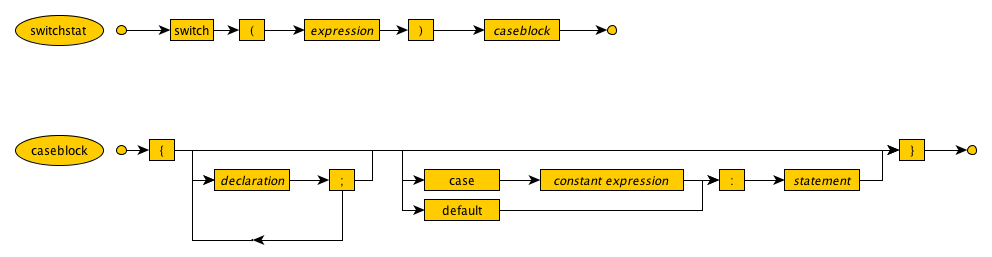
\includegraphics[scale=.5]{SyntaxDiagramCSwitchStatement.png}
	
	Rewrite this rule in the form of classical formal language grammar notation.
	
	\begin{otherlanguage}{german}
		Gegeben sei obiges Syntax Diagramm. Schreiben Sie dieses in die klassische Grammatik-Notation um.
	\end{otherlanguage}
	
\question{\bf Java Method Definition}
Give the grammar of the Java method definition in EBNF. You may use the non-terminals ``Statement'', ``Type'', and ``Identifier". Split the grammar into useful non-terminals. MethodDefinition, MethodHead, MethodBody, ParameterList, OneParameter could be useful candidates.

\begin{otherlanguage}{german}
	Geben Sie die Grammatik für Methodendefinition in JAVA in EBNF an. Sie dürfen die Non-Terminal-Symbole ``Statement'', ``Type'' und ``Identifier'' als gegeben voraussetzen und brauchen diese nicht weiter zu definieren. Teilen Sie Ihre Grammatik in vernünftige Non-Terminale auf. MethodDefinition, MethodHead, MethodBody, ParameterList, OneParameter könnten vernünftige Kandidaten sein.
\end{otherlanguage}

\question {\bf Simple Protocol}
A simple protocol to transmit data from sender to a receiver has a header followed by one or more data fragments. The header contains a version string which starts with the character ``V'' followed by a max. two-digit number. Optionally an arbitrary number of further two digits number may follow (sub-version identifier) which are separated by ``.'' (dots). The string {\tt V2.01.4.00} would be a valid version string. After this an optional sender address may follow. The header is finished by the receiver's address. Both addresses are 6 digit numbers, where the sender address is pre-fixed by an ``S'' and the receiver address is pre-fixed by a ``D''.

A data fragment starts with a max. three digit number denoting the size of the following data. The data itself is a sequence of one or more characters (obviously as many as given in the data size field before). The data fragment is finished by a flag ``T'' or ``F'' indicating whether a next data fragment follows or not.

Describe this protocol in form of Wirth's EBNF. You may assume to have the terminal classes ``digit'' and ``char''.

\begin{otherlanguage}{german}
Ein einfaches Protokoll zur Datenübertragung von einem Sender zu einem Empfänger besteht aus einem Header und einem oder mehreren Datenfragmenten. Der Header startet mit einem Versionsstring, der mit dem Zeichen ``V'' beginnt und von einer maximal zweistelligen Zahl gefolgt wird. Eventuell können noch weitere max. zweistellige Zahlen folgen (Bezeichner für Unterversionen), welche durch einen ``.'' (Punkt) voneinander getrennt sind. Der String {\tt V2.01.4.00} wäre ein gültiger Versionsstring. Nach dem Versionsstring folgt optional eine Senderadresse. Der Header wird von der Empfängeradresse abgeschlossen. Beide Adressen sind sechsstellige Zahlen, wobei die Senderadresse ein ``S'' und die Empfängeradresse ein ``D'' vorangestellt hat.

Ein Datenfragment startet mit einer maximal dreistelligen Zahl, welche die Anzahl der Zeichen der nun folgenden Daten beschreibt. Die Daten selbst sind eine Sequenz von einem oder mehreren Zeichen (characters), offensichtlich so viele, wie vorher bei der Anzahl angegeben wurden. Das Datenfragment wird von einem Flag ``T'' oder ``F'' abgeschlossen, welches anzeigt, ob noch ein weiteres Fragment folgt oder nicht.

Beschreiben Sie dieses Protokoll mit Hilfe der Wirth'schen EBNF. Sie dürfen die Terminalklassen ``digit'' und ``char'' voraussetzen.
\end{otherlanguage}

\begin{solution}

	\begin{grammar}
		Message & = & Header DataFragments. \\
		Header &=& Version TotalLength [SourceAddress] DestinationAddress.\\
		Version &=& ``V''digit [digit] \{``.'' digit[digit]\}. \\
		SourceAddress &=& ``S'' Address. \\
		DestinationAddress &=& ``D'' Address. \\
		Address &=& digit digit digit digit digit digit. \\
		DataFragments &=& DataFragment \{DataFragment\}.\\
		DataFragment &=& DataSize Data IsLastFragment. \\
		DataSize &=& digit [digit [digit]]. \\
		Data &=& char \{char\}. \\
		IsLastFragment &=& ``T'' $|$ ``F''.
	\end{grammar}
\end{solution}

\question{\bf US Phone Number}
Write an EBNF description for {\em PhoneNumber}, which describes telephone numbers written according to the following specifications.

\begin{itemize}
	\item Normal: a three digit exchange, followed by a dash, followed by a four digit number: e.g., 555-1212
	
	\item Long Distance: a 1, followed by a dash, followed by a three digit area code enclosed in parentheses, followed by a three digit exchange, followed by a dash, followed by a four digit number: e.g., 1-(800)555-1212
	
	\item Interoffice: an 8 followed by a dash, followed by a four digit number: e.g., 8-2404
\end{itemize}
The description should be compact, and each rule should be well named.


\end{questions}
\end{document}